%% Normalidade Contextual em APIs -- versão 10 em inglês (tradução de main-v10.tex; figuras em figuras_en, geradas por v10/figuras_v10_en.py)
%% Classe acmart (sigconf), compatível com Overleaf (pdfLaTeX, XeLaTeX ou LuaLaTeX).
\documentclass[sigconf,nonacm]{acmart}

\usepackage{booktabs}
\usepackage{amsmath}
\usepackage{xspace}
\usepackage{fancyvrb}

\citestyle{acmauthoryear}
\settopmatter{printacmref=false, printfolios=true}
\setlength{\emergencystretch}{1.5em}

\newcommand{\Normal}{\textsc{Normal}\xspace}
\newcommand{\Residual}{\textsc{Residual}\xspace}

\begin{document}

\title{Contextual Normality in APIs: Characterizing Regimes from Access Logs to Support Incident Analysis}

\author{Diego Paz Casagrande}
\affiliation{%
  \institution{Universidade de Brasília}
  \city{Brasília}
  \state{DF}
  \country{Brazil}}

\renewcommand{\shortauthors}{D. P. Casagrande}

\begin{abstract}
When an incident is opened, one of the operator's first questions is whether the APIs involved are operating normally and, if not, which indicator has departed from its usual pattern. The answer is not trivial, because an API's behavior varies legitimately with the time of day, the calendar, and batch processing, and it changes over the months. This work investigates whether API Access Logs (AALs) aggregated per minute make it possible to answer, at the moment the incident is registered, whether each API resource is in one of its normal regimes (Normal) or outside them (Residual); which indicator is responsible: business errors (4xx), system errors (5xx), or latency; and since when. Following CRISP-DM, we propose a contextual normality profile per resource, with a separate limit for each indicator calibrated by cross-validation, and a backward expansion in bands from 15 min to 4 h to estimate the onset of the deviation. On 5.6 million records from 12 production resources between May and September 2026, statistical tests confirmed regimes tied to the hour of the day. In 12,157 simulated queries in August and September, the decision on the 15 minutes before registration had a specificity of 97.1\% and pointed to the correct indicator in 96.5\% of the detected cases; the actual onset fell within the estimated zone in 91.7\% of them. Sensitivity was 39\%: high for system errors (up to 88\%), low for business errors and, for latency, 36\% to 61\% for 4-fold and 10-fold degradations. A 1-month history outperformed a 3-month history, indicating that API behavior changes over time and that frequent retraining is preferable to a long history.
\end{abstract}

\keywords{Data Mining; API Access Log; Contextual Normality; Incident Analysis; CRISP-DM; Operational Regimes.}

\maketitle

%% =====================================================================
\section{Introduction}

The architecture of modern systems has established APIs (\emph{Application Programming Interfaces}) as a fundamental integration mechanism in distributed systems. In large corporate environments, APIs mediate everything from requests by external clients to transactions between legacy and modern systems. At Banco do Brasil, about 30,000 APIs run daily, connecting business solutions that combine cloud platforms and \emph{mainframe}.

\subsection{Context}

Requests processed by API gateways generate records with the execution time, the resource accessed, the response code, the processing time, and the consumer. In this study, these records are called \emph{API Access Logs} (AALs): the record generated by the gateway for the requests it processes, distinct from the \emph{execution log} and from the application log. AALs are available in a standardized form for a broad set of APIs, without specific instrumentation in the code. An API exposes one or more resources, also called \emph{endpoints}, which are the executable unit and the unit of analysis of this work; the terms are treated here as synonyms, and \emph{resource} is adopted.

The operational behavior of an API is not necessarily stationary. Volume, latency, and the proportion of errors vary with the time of day, the day of the week, batch processing, and maintenance windows. A high error rate may be normal at the turn of the day, just as higher latency may indicate degradation or merely an expected increase in request volume; an abrupt drop in traffic may indicate unavailability or the end of a service period.

\subsection{Problem}
When an incident is registered, the operator needs to put the situation into semantic context and answer, for each API involved: \emph{was the period before the registration within the normal behavior expected for that moment?} If it was not, it also matters to know which metrics deviated, such as business errors (4xx range), system errors (5xx range), or latency, and since when the deviation has been occurring. As complementary information, it is useful to know whether the impact is widespread or concentrated in one specific client application with enough volume to change the state of the API. An error spread across all consumers suggests a problem in the provider.

Today this answer depends on consulting several tools and on knowing the typical behavior of each API and resource~\citep{kataria2025isre}. Approaches with fixed limits or with a single normality profile do not distinguish legitimate variation, such as a batch at midnight or lower volume on Sunday, from a real deviation.

From a data mining standpoint, the problem consists of: (1) characterizing the normal regimes of each resource from AALs aggregated in windows; (2) classifying the period immediately before the registration of an incident into two states: \Normal (within some normal regime expected for that context) or \Residual (everything else); and (3) when \Residual, identifying which parameter deviated, this being the responsible indicator, and since when the deviation has been occurring.


\subsection{Motivation}
This work complements a master's project on multi-agent systems to support incident handling. Recent literature shows agents specialized in different data sources, coordinated for triage and analysis~\citep{yu2025triangle,luo2025opsagent,kataria2025isre}. One of these agents needs a reliable and explainable source on the behavior of the APIs. The focus is neither real-time monitoring nor root cause identification, but \emph{context information at the moment of the incident}: stating whether each resource is in a normal regime and, if not, which indicator is impacted and since when. This information feeds the operator through a specialist agent and contributes to the analysis of what happened, delivering a semantic context grounded in data mining. The project hypothesis is that preprocessed and structured evidence reduces the amount of raw data the agent needs to go through, saving computational resources and avoiding hallucinations; the present work evaluates the quality of this evidence, not the performance of the agent that consumes it.

\subsection{Objectives}
\textbf{General objective:} to characterize the normal regimes of each API resource from Access Logs aggregated per minute and, at the moment an incident is registered, to report whether the resource is in a \Normal regime and, if not, which indicator was impacted and since when.

\textbf{Specific objectives:}
\begin{itemize}
  \item Verify whether each resource exhibits several normal regimes tied to the context (hour and day type).
  \item Build a normality profile per resource and context and an explainable \Normal or \Residual decision rule.
  \item Identify the responsible indicator (4xx, 5xx, latency) and estimate the onset of the deviation.
  \item Evaluate the method on simulated incident scenarios over two months and compare it with simple baselines.
  \item Evaluate how much history the profile needs (3 months or 1 month).
  \item Provide the information in a structured format for an agent or operator.
\end{itemize}

\subsection{Research questions}
\begin{itemize}
  \item \textbf{RQ1.} Do aggregated AALs make it possible to characterize the normal regimes of each resource and decide, at the moment of registration, whether the resource is in a \Normal regime?
  \item \textbf{RQ2.} When the resource is not in a \Normal regime, does the method correctly identify the responsible indicator (4xx, 5xx, latency) and the onset of the deviation?
  \item \textbf{RQ3.} Which period before the registration (15, 30, or 60~min) is most suitable for the decision, and how does the interval between the onset of the degradation and the registration affect the result?
  \item \textbf{RQ4.} Does a longer history (3 months) produce a better profile than the recent history (1 month)?
\end{itemize}

\subsection{Contributions and organization}
The contributions are: (i) a traceable characterization of the regimes of 12 production API resources over five months; (ii) a simple and explainable method, without labels, that decides the state of a resource at the moment of registration and points to the impacted indicator; (iii) an onset estimate by backward expansion; (iv) an evaluation protocol with simulated incident scenarios over two months; and (v) evidence that, on these data, recent history is more useful than a long one. Section~\ref{sec:correlatos} discusses related work; Section~\ref{sec:metodologia}, the methodology; Section~\ref{sec:resultados}, the results; Section~\ref{sec:discussao}, the discussion; Section~\ref{sec:ameacas}, the threats to validity; and Section~\ref{sec:conclusao} concludes.

%% =====================================================================
\section{Related work}\label{sec:correlatos}

The related literature is organized into four fronts and assessed according to four criteria that follow from the problem addressed here: (i) the data source required; (ii) how normality is treated, that is, whether the expected behavior is single or conditioned on context; (iii) the type of output produced, a score or an explanation; and (iv) the need for labels or additional instrumentation. Table~\ref{tab:correlatos} summarizes the comparison.

\begin{table*}[t]
  \caption{Comparison with related work according to the four criteria.}
  \label{tab:correlatos}
  \small
  \begin{tabular}{p{0.17\textwidth}p{0.19\textwidth}p{0.17\textwidth}p{0.2\textwidth}p{0.18\textwidth}}
    \toprule
    Work & Data source & Normality & Output & Labels or instrumentation \\
    \midrule
    DeepLog, LogAnomaly & system log sequences & single & score or binary label & application log with \emph{templates} \\
    SPOT/DSPOT & univariate time series & adapted over time & threshold and alarm & --- \\
    USAD & multivariate series & single & score & clean training period \\
    \citet{wang2025crosssystem} & \emph{traces} & single per system & anomaly category & \emph{traces}; labeled examples \\
    DeepTraLog, GAMMA & \emph{traces}, logs, and metrics & single & score or localization & distributed instrumentation \\
    Triangle, OpsAgent, ISRE & multiple incident sources & not modeled (consumes evidence) & triage or diagnosis & integration with the sources \\
    \midrule
    \textbf{This work} & AAL aggregated per minute & family of regimes per context & state, indicator, and onset, with explanation & nothing beyond the AAL; no labels \\
    \bottomrule
  \end{tabular}
\end{table*}

\subsection{Log analysis and mining}
\citet{du2017deeplog} proposed DeepLog, which models sequences of log events with LSTM networks and flags as anomalous every sequence that is unlikely under the learned model. \citet{meng2019loganomaly} extended this line with LogAnomaly, combining the semantic information of the \emph{templates} with the detection of sequential and quantitative anomalies. Both support the premise we also adopt: logs carry enough information to characterize behavior, without dedicated instrumentation.

The differences, however, are decisive for the problem addressed here. First, the unit of analysis is the sequence of system log events, which presupposes stable \emph{templates} and access to the application log; the AAL is a per-minute aggregate, with no event order and no text from which to extract \emph{templates}. Second, and more importantly, normality in these models is single: a distribution of normal sequences is learned, and whatever departs from it is anomalous. A batch at midnight or a maintenance window produce legitimate patterns that a model without context tends to treat as deviations, unless the time of day enters implicitly as an attribute, which these works do not explore. Third, the output is a score or a binary label. For the operator who has just opened an incident, knowing that the sequence is improbable does not answer which indicator departed from the pattern or since when.

\subsection{Normality and time series}
\citet{siffer2017spot} proposed SPOT and its \emph{drift} variant, DSPOT, which calibrate thresholds from the tail of the distribution using Extreme Value Theory, with adaptation to non-stationary series. It is the work closest to ours in spirit: both recognize that the threshold cannot be fixed and derive it from the observed distribution itself, without labels. DSPOT adapts the threshold \emph{over time}, following the series; the contextual profile treats it as a function of variables known \emph{a priori}, hour and day type. The practical consequence is that temporal adaptation absorbs a slow degradation as if it were the new normal, whereas conditioning on context preserves the reference of the same hour on previous days. On the other hand, DSPOT does not require the relevant contexts to be known in advance, which is an advantage in domains where seasonality is not obvious.

\citet{audibert2020usad} proposed USAD, based on autoencoders for multivariate series. The method is more expressive than ours and captures dependencies between indicators. There is also the matter of training, which presupposes a period free of anomalies; in production data without a labeled incident history, such as ours, this assumption cannot be verified.

\citet{wang2025crosssystem} document the difficulty of transferring detection models between different systems, even with meta-learning. The finding is relevant as a negative justification for our choice of fitting one profile per resource: if transfer between systems is difficult, transfer between resources with very different traffic profiles in our data would hardly be easier. The trade-off is that per-resource profiles do not generalize to new resources, which need to accumulate history before being evaluated; our results in September, with resources with short histories, show this cost.


\subsection{Behavioral modeling of microservices}
DeepTraLog~\citep{zhang2022deeptralog} combines \emph{traces} and logs in an event graph and learns, with graph neural networks, the expected structure of a request; GAMMA~\citep{somashekar2024gamma} locates performance bottlenecks by exploiting the dependency topology between services. Both deliver something the present work does not: localization, that is, an indication of \emph{where} in the call chain the problem manifests itself.

This gain has a prerequisite. Both presuppose distributed \emph{traces} or correlated infrastructure metrics, which require consistent instrumentation in all services of the chain. In heterogeneous corporate environments, which combine cloud platforms and legacy systems, this coverage is uneven. The AAL has the opposite property: it is poor in structure, because it does not see beyond the \emph{gateway}, but it is uniformly available. The two approaches are therefore complementary, not competing.


\subsection{Incidents and multi-agent systems}
Triangle~\citep{yu2025triangle} organizes multiple agents for incident triage; OpsAgent~\citep{luo2025opsagent} and the work of \citet{kataria2025isre} coordinate agents specialized in different sources for incident analysis and root cause determination. These systems shift the problem. The challenge is no longer the detection algorithm but the quality and readability of the evidence each agent consumes.

It is at this point that the evaluation of these works leaves an open question. The competence of the multi-agent system is measured end to end (triage accuracy, root cause accuracy), without isolating the contribution of each source or characterizing its error regime.

\subsection{Synthesis and gap}
The comparison reveals a pattern: the works that dispense with labels treat normality as single or as something that adapts over time, but not as a family of coexisting legitimate regimes; those that model behavior richly enough to distinguish situations depend on sources beyond the AAL; and those that produce actionable explanations do so at the level of the agent system, taking as given the evidence they receive. None of them investigates, exclusively from the AAL, whether the same resource exhibits several normal regimes and whether this characterization can inform, at the moment an incident is registered, the state of the resource, the impacted indicator, and the onset of the deviation.

%% =====================================================================
\section{Methodology}\label{sec:metodologia}

The work follows CRISP-DM~\citep{chapman2000crispdm,wirth2000crispdm}. Each phase was implemented in a Jupyter \emph{notebook} with explicit parameters and fixed seeds for all random draws, so that the scenarios and the clusterings are reproducible (Table~\ref{tab:fases}). The analysis is always per resource. Techniques that are easy to explain were chosen, all available in widely used Python libraries, such as pandas, SciPy, and scikit-learn~\citep{pedregosa2011sklearn}.


\begin{table}[t]
  \caption{CRISP-DM phases, notebooks, and techniques. Phases repeat because
  the process is iterative; the order follows that of the notebooks.}
  \label{tab:fases}
  \small
  \begin{tabular}{p{0.2\columnwidth}p{0.7\columnwidth}}
    \toprule
    Phase & Notebook: content (technique) \\
    \midrule
    Business, Data & 01: problem, success criteria, quality, and monthly evolution of the data \\
    Preparation & 02: consolidation, attributes per window, p95 latency (percentile) \\
    Data, Modeling & 03: regimes (Kruskal-Wallis with Bonferroni; k-means with silhouette) \\
    Modeling & 04: contextual profile (median/MAD); limit per indicator (percentile, cross-validation), per test month and history \\
    Preparation & 05: incident scenarios (fault injection) \\
    Evaluation & 06: state, indicator, onset (backward expansion); history; Wilson CI, McNemar \\
    Deployment & 07: structured query for the agent \\
    \bottomrule
  \end{tabular}
\end{table}

\subsection{Business understanding}
The decision supported is: \emph{at the moment the incident is registered, is the resource in a normal regime? If not, which indicator was impacted (4xx errors, 5xx errors, latency) and since when?} The scope (specific consumer or widespread) is complementary information. The success criteria were defined before modeling (Table~\ref{tab:criterios}). Since there was no incident history, the evaluation uses simulated scenarios with injected faults.

\subsection{Data understanding}
The dataset contains production AALs from 12 resources of different APIs, identified here as E01 to E12 (in decreasing order of volume in August). Each record is a per-minute aggregate by execution date and time, resource, HTTP response code (status code), and client, with the total number of executions in the minute and the mean time of these executions. Since per-minute temporal aggregation is already available in this format, we chose not to use the per-execution records, which does not prevent using the raw records to perform this aggregation and feed it into this process. The client identifier was anonymized with seeded SHA-256, with no payloads or personal data. Timestamps, in UTC, were converted to Brasília time (UTC-3) before any temporal cut.

There are 5,602,126 records from May 1, 2026, 00:00 to September 19, 2026, 23:59 (Brasília time), with 1,976 distinct clients. Successful responses (HTTP response code = 2xx) account for 87.6\% of the transactions; business errors (HTTP response code = 4xx), 12.2\%; and system errors (HTTP response code = 5xx), 0.21\%. Coverage varies: seven resources have data since May; E04, since May 25; five (E02, E03, E06, E10, E11), only since July 16; and four (E02, E03, E06, E11) stop on September 3. The volume of executions per 15 min ranges from 47 transactions (E11) to 2,239 (E02). These numbers show the heterogeneity of the dataset across resources.

\paragraph{Monthly evolution.} Behavior changes over the months. Between May and September, the mean daily volume grows by 35\% to 60\% in several resources (E07, E08, E12), and the business error rate shifts level: in E02, it goes from 32\% (July) to 45\% (August) and 62\% (September); in E04, from 0.5\% (May) to 13\% (August). This change motivates question RQ4.

\subsection{Data preparation}
Repeated keys were consolidated (sum of volume and weighted mean latency). The records were aggregated into 1~h windows (29,509 resource $\times$ hour windows), which form the basis of the normality profile. The decision uses four indicators (Table~\ref{tab:atributos}). The \emph{context} of each window is the pair (day type, hour), with day type \emph{business} or \emph{non-business} (Saturday, Sunday, and holidays).

\paragraph{p95 latency.} Since there is no per-request latency, the p95 is the 95th percentile of the mean latencies per minute $\times$ client of 2xx responses, weighted by the number of executions. It is a p95 \emph{of the means}, not of the requests, and tends to underestimate the real tail; but it is consistent across periods and sensitive to degradations that affect only part of the minutes or of the consumers. At the median, it is 1.42 times the mean latency.


\begin{table}[t]
  \caption{Indicators used in the decision and unfavorable direction.}
  \label{tab:atributos}
  \small
  \begin{tabular}{p{0.2\columnwidth}p{0.52\columnwidth}p{0.16\columnwidth}}
    \toprule
    Indicator & Definition & Direction \\
    \midrule
    volume & $\log(1+$transactions$)$, on the hourly scale & increase and drop \\
    4xx errors & 4xx transactions / total (business errors) & increase \\
    5xx errors & 5xx transactions / total (system errors) & increase \\
    p95 latency & $\log(1+$p95 of the means per minute$\times$client$)$ & increase \\
    \bottomrule
  \end{tabular}
\end{table}

\subsection{Modeling}

\paragraph{Regimes (descriptive).} The Kruskal-Wallis test~\citep{kruskal1952ranks}, with Bonferroni correction~\citep{dunn1961multiple}, checks whether each indicator changes across the 24 hours of business days. For each resource, k-means~\citep{lloyd1982kmeans} clusters the 1~h windows from May to August using only the indicators, standardized and capped at the resource's 1st and 99th percentiles (over a four-month period, isolated spikes would form their own clusters with less than 0.5\% of the hours). The number of regimes, $k\in[2,8]$, is chosen by the silhouette coefficient~\citep{rousseeuw1987silhouette}. The context does not enter the clustering, so that the regime--context relationship is a finding rather than an input; it is used afterwards to name each regime (volume level, day type, and hours in which it predominates). k-means is descriptive: the decision uses the contextual profile.

\paragraph{Contextual normality profile.} For each resource, context, and indicator, the profile stores the historical median and a robust scale of variation, computed over the one-hour windows of the history. The scale is obtained from the median absolute deviation (MAD), multiplied by 1.4826 to make it comparable to the standard deviation, and respects a minimum value to avoid division by values close to zero. For each period evaluated, the observed value is compared with the median expected for that resource and context, and this difference is divided by the robust scale. The result indicates by how many scales of normal variation the indicator departs from the expected value. For volume, both increases and drops are considered unfavorable; for 4xx errors, 5xx errors, and latency, only increases count as deviations. Periods of 15 and 30 minutes use the same one-hour profile: volume is converted to the hourly scale, and the rates and the p95 are used directly.

\paragraph{Limit per indicator.} The indicators have very different variabilities; in some resources the 4xx rate has frequent real spikes. Therefore, each indicator has its own limit in the resource, $L_{r,a}=\max\{3,\ Q_{0.99}(d_a)\}$: the 99th percentile of its deviations in the history, computed out of sample. The limit is recomputed for each period size (15, 30, and 60~min), because short periods vary more. The period is \Residual if any indicator exceeds its limit ($d_a/L_{r,a}>1$); the \textbf{responsible indicator} is the one that exceeded it the most, in multiples of the limit.

\paragraph{History and leakage-free calibration.} For each test month (August; September 1 to 19), the profile and the limits are fitted only with earlier data, in two histories: \emph{3 months} (main; May to July for August and June to August for September) and \emph{1 month} (the previous month). The out-of-sample deviations come from cross-validation with four contiguous time blocks within the history: the profile is fitted on three blocks and evaluates the remaining one. With this rule, about 3\% of the periods in the history are \Residual.

\paragraph{Query at registration and estimated onset (backward expansion).} At the registration time $t$, the method looks back from $t$ in disjoint bands increasingly far away: 0--15, 15--30, and 30--60~min and then hour by hour up to 4~h. The most recent band, $[t-15\,\text{min}, t)$, defines the \emph{state at registration} and the responsible indicator. If it is \Residual, the search continues backward and stops at the first \Normal band; the onset is estimated between the start of the last residual band and the end of that normal band (``started between 30 and 120~min before registration''). All bands are compared with the same 1~h profile: volume is converted to the hourly scale, and the rates and the p95 are used directly. Since short bands vary more, each band size receives its own limits, calibrated in the same way.

\paragraph{Scope (complementary).} For 4xx or 5xx errors, the deviation is attributed to a \emph{specific consumer} when the client with the most errors concentrates at least 80\% of them and this share exceeds its share of the volume by at least 20 percentage points; otherwise, it is \emph{widespread}. Resources with fewer than three active clients are left undetermined.

\subsection{Evaluation}

\paragraph{Incident scenarios.} Each scenario simulates an incident: a degradation starts at $t_0$ and the incident is registered at $t=t_0+\Delta$, with delay $\Delta\in\{15,30,60,120\}$~min. The registration time is drawn within the test month. A month's test includes the resources with at least 28 days of data in the previous month: 7 resources in August and all 12 in September. The faults (Table~\ref{tab:falhas}) are applied to the per-minute $\times$ client records and then re-aggregated, so that the indicators and the scope react as in a real fault. Five scenarios were generated per resource $\times$ month $\times$ cause $\times$ intensity $\times$ delay (6,080 incidents, of which 3 fell in intervals with no traffic at all in the resource, where the fault does not manifest itself, and were excluded) and 6,080 control queries, at times without injected faults.

\begin{table}[t]
  \caption{Injected causes.}
  \label{tab:falhas}
  \small
  \begin{tabular}{p{0.26\columnwidth}p{0.64\columnwidth}}
    \toprule
    Cause & Intensity (low / medium / high / very high) \\
    \midrule
    Widespread 4xx & 5\% / 15\% / 40\% of the 2xx become 400 \\
    4xx from 1 consumer & 30\% / 60\% / 90\% of the consumer's 2xx become 400 \\
    Widespread 5xx & 5\% / 15\% / 40\% of the 2xx become 503 \\
    5xx from 1 consumer & 30\% / 60\% / 90\% of the consumer's 2xx become 503 \\
    Latency & execution time $\times$1.5 / $\times$2.5 / $\times$4 / $\times$10 \\
    \bottomrule
  \end{tabular}
  \par\smallskip\footnotesize The affected consumer is drawn with probability proportional to its volume.
\end{table}

\paragraph{Latency $\times$10.} Since latency comes from per-minute means, a few slow requests raise the value considerably. In the May to August history, the hourly p95 exceeded 10 times the median of its context in 0.78\% of the hours (99.9th percentile: 25 times; maximum: 68 times). Latency degradations relevant to an incident tend to be of this size, so the ``very high'' intensity ($\times$10) was included for latency. The lower intensities were kept to show the limit of the method.

\paragraph{Metrics.} For each scenario, the query is made at the registration time, as described above. The metrics are: \emph{sensitivity} (incidents with \Residual output); \emph{specificity} (controls with \Normal output); \emph{indicator accuracy} (indicator pointed out equal to that of the injected cause, among those detected); \emph{onset hit} (actual onset within the zone estimated by the backward expansion); and \emph{scope accuracy}. ``Medium/high'' refers to the medium and high intensities, without latency $\times$10, for comparison with earlier versions of the study. Proportions have 95\% Wilson confidence intervals~\citep{wilson1927probable}.

\paragraph{Baselines.} The baselines assess whether the contextual profile adds value to the decision. The first is the \emph{global z-score}, which uses the same logic of median, MAD, and limits per indicator but ignores hour and day type: each resource has a single historical reference for each indicator. The second is the \emph{previous week}, which compares the evaluated period with the same time interval seven days earlier, exploiting weekly periodicity without building a broader statistical profile. The three methods use the same treatment of limits and calibration, so that the comparison isolates the effect of the reference strategy.

The comparison between methods uses McNemar's exact test~\citep{mcnemar1947note} on the state hits in the same simulated scenarios. The test considers only the cases in which the methods diverge: those in which the contextual profile is right and the baseline is wrong, and those in which the opposite occurs. A small $p$ value indicates evidence of a statistically significant difference between the methods. The same test compares the profiles fitted with 3-month and 1-month histories, since both are applied to the same scenarios.

\paragraph{Experiments.} \textbf{Exp.~1} characterizes the regimes of each resource (Kruskal-Wallis and k-means). \textbf{Exp.~2} evaluates the state at registration: sensitivity, specificity, and comparison with the baselines. \textbf{Exp.~3} evaluates the query when the resource is \Residual: responsible indicator, onset estimated by the backward expansion, and scope. \textbf{Exp.~4} compares the 3-month and 1-month histories.

%% =====================================================================
\section{Results}\label{sec:resultados}

\subsection{Exp.~1: normal regimes per resource (RQ1)}

Figure~\ref{fig:perfis} shows typical hourly profiles: a batch at the turn of the day and at 18h on business days (E01), a batch at 15--16h (E05), and a business-hours pattern on business days that disappears on non-business days (E02, E12). The heat map (Figure~\ref{fig:mapa}) confirms that each resource has its own hourly signature of volume and latency. On business days, 96\% of the Kruskal-Wallis tests (resource $\times$ indicator) were significant after Bonferroni. The median effect ($\varepsilon^2$) was large for volume (0.40), 4xx errors (0.28), and p95 latency (0.25), and small for 5xx errors (0.05), which are rare on normal days.

\begin{figure*}[t]
  \centering
  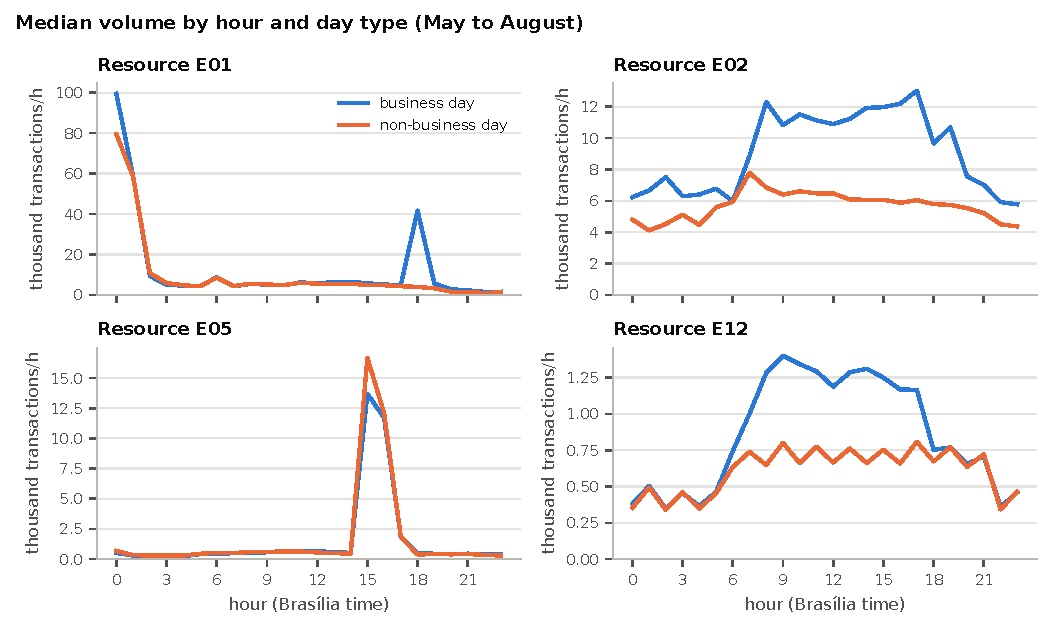
\includegraphics[width=0.9\textwidth]{figuras_en/fig_perfis_volume.pdf}
  \caption{Median volume by hour and day type (May to August), in four resources.}
  \label{fig:perfis}
\end{figure*}

\begin{figure*}[t]
  \centering
  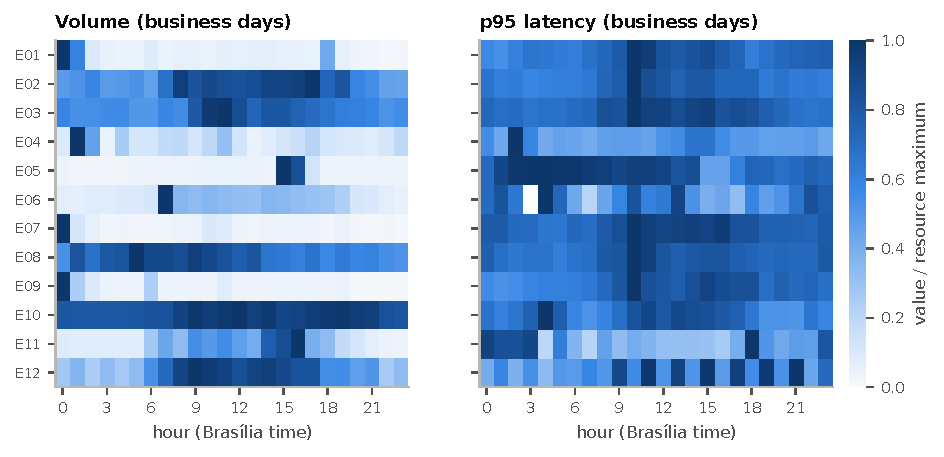
\includegraphics[width=0.85\textwidth]{figuras_en/fig_mapa_calor.pdf}
  \caption{Median volume and p95 latency by hour on business days, normalized by the maximum of each resource.}
  \label{fig:mapa}
\end{figure*}

k-means found 2 to 8 regimes per resource (median 3; mean silhouette 0.51; Table~\ref{tab:recursos}). Figure~\ref{fig:regimes} illustrates E02: a high-volume regime from 8 to 19h on business days, a medium-volume one for the rest of the time, a low-volume one on non-business days, a sporadic regime of high volume and latency, and a regime at 0h with a high 5xx rate. This last one is \emph{normal} for that hour: it is the kind of legitimate variation that a fixed limit would treat as a failure.

\begin{figure*}[t]
  \centering
  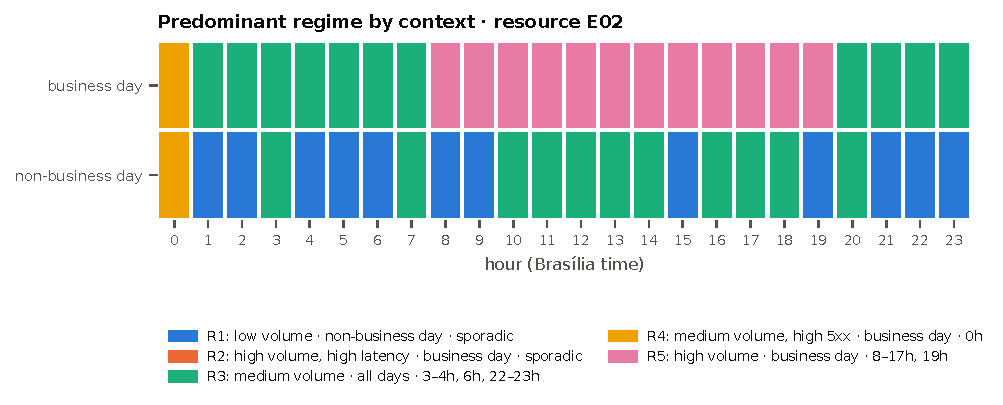
\includegraphics[width=0.85\textwidth]{figuras_en/fig_regimes_contexto.pdf}
  \caption{Predominant regime (k-means with the indicators) by day type and hour in resource E02.}
  \label{fig:regimes}
\end{figure*}

\begin{table*}[t]
  \caption{Summary per resource: share of volume, clients, median transactions per 15~min, regimes (Exp.~1), test months, and results at registration (Exp.~2 and 3; 15~min band, 3-month history).}
  \label{tab:recursos}
  \small
  \begin{tabular}{lrrrrrcrrrr}
    \toprule
    Resource & Vol. (\%) & Clients & Trans./15 min & Regimes ($k$) & Silhouette & Test & Sens. & Sens. medium/high & Spec. & Indicator accuracy \\
    \midrule
    E01 & 47.2 & 38  & 1,212 & 3 & 0.36 & Aug, Sep & 0.60 & 0.66 & 0.97 & 0.98 \\
    E02 & 12.0 & 555 & 2,239 & 5 & 0.55 & Sep & 0.18 & 0.26 & 0.98 & 0.84 \\
    E03 & 3.1  & 246 & 498   & 4 & 0.52 & Sep & 0.25 & 0.33 & 0.95 & 0.87 \\
    E04 & 4.9  & 24  & 149   & 2 & 0.54 & Aug, Sep & 0.36 & 0.40 & 0.96 & 0.94 \\
    E05 & 6.0  & 19  & 113   & 2 & 0.78 & Aug, Sep & 0.44 & 0.43 & 0.97 & 0.98 \\
    E06 & 2.4  & 787 & 290   & 2 & 0.64 & Sep & 0.09 & 0.10 & 0.94 & 0.69 \\
    E07 & 5.7  & 36  & 123   & 2 & 0.63 & Aug, Sep & 0.42 & 0.42 & 0.98 & 0.97 \\
    E08 & 5.9  & 39  & 279   & 5 & 0.35 & Aug, Sep & 0.49 & 0.55 & 0.99 & 0.99 \\
    E09 & 5.6  & 30  & 132   & 3 & 0.66 & Aug, Sep & 0.63 & 0.70 & 0.97 & 0.99 \\
    E10 & 2.2  & 2   & 260   & 8 & 0.29 & Sep & 0.06 & 0.06 & 1.00 & 1.00 \\
    E11 & 2.0  & 625 & 47    & 3 & 0.55 & Sep & 0.20 & 0.22 & 0.99 & 0.97 \\
    E12 & 2.9  & 831 & 174   & 4 & 0.29 & Aug, Sep & 0.40 & 0.49 & 0.96 & 0.97 \\
    \bottomrule
  \end{tabular}
\end{table*}

\paragraph{Limits per indicator.} The limits (Figure~\ref{fig:limites}) range from 3 to 86 in $z$. High limits reveal indicators with frequent real spikes in the history: 4xx errors in E04 (86), E05 (81), and E07 (56); 5xx errors in E10 and E12 (about 20); and p95 latency in E02 (38) and E03 (23). In these cases, only large deviations of that indicator are flagged as \Residual. In the June to August history, out of sample, 3.3\% of the 1~h windows were residual, with latency (201 windows), volume (200), 4xx errors (191), and 5xx errors (101) as responsible indicators.

\begin{figure*}[t]
  \centering
  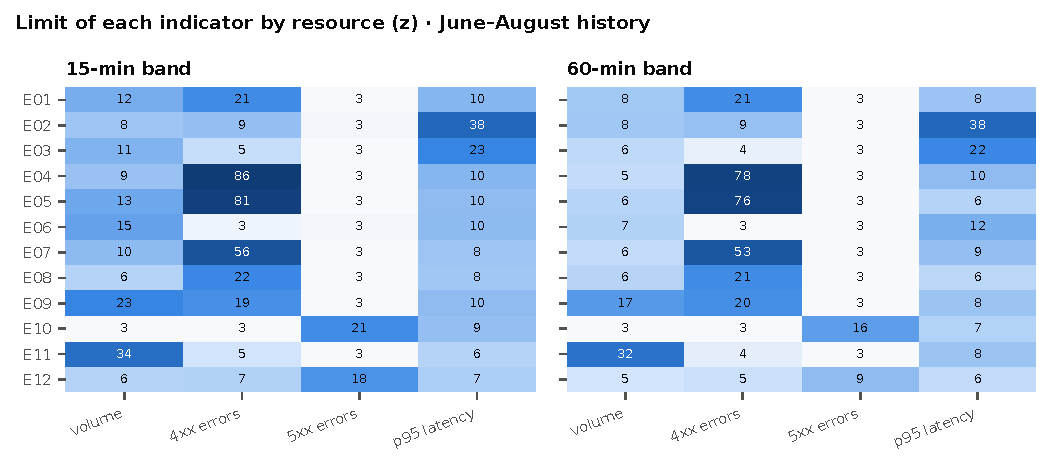
\includegraphics[width=0.85\textwidth]{figuras_en/fig_limites.pdf}
  \caption{Limit of each indicator per resource ($z$, out-of-sample 99th percentile, minimum 3), for periods of 15 and 60~min; June to August history.}
  \label{fig:limites}
\end{figure*}

\subsection{Exp.~2: state at the moment of registration (RQ1 and RQ3)}
Table~\ref{tab:metodos} and Figure~\ref{fig:metodos} summarize the decision. With the 15~min band, the contextual profile correctly classified 97.1\% of the controls as \Normal and flagged 39.3\% of the incidents as \Residual (43.2\% at medium and high intensities). In state hits, it ties with both baselines in the 15 min band (McNemar: $p = 0.12$ against the global z-score; $p = 0.75$ against the previous week) and outperforms the global z-score in the 30 min band ($p = 0.009$). This last difference should be read with caution: the methods operate at different points of the alarm curve, and the state hit, with incidents and controls in approximately equal proportion by construction, is equivalent to the mean of sensitivity and specificity. The comparison paired by alarm rate is the appropriate reading, and in it the contextual profile does not detect more than the baselines.

\begin{table*}[t]
  \caption{Exp.~2: state at registration by method and band before registration, in \% (95\% Wilson CI in brackets). 3-month history; 6,077 incidents and 6,080 controls.}
  \label{tab:metodos}
  \small
  \begin{tabular}{llccc}
    \toprule
    Method & Band $L$ & Sensitivity & Sensitivity (medium/high) & Specificity \\
    \midrule
    \textbf{Contextual profile (proposed)} & 15 min & \textbf{39.3} [38.1, 40.5] & \textbf{43.2} [41.7, 44.8] & 97.1 [96.6, 97.5] \\
     & 30 min & 39.0 [37.8, 40.2] & 43.4 [41.9, 45.0] & 97.0 [96.5, 97.4] \\
     & 60 min & 36.2 [35.0, 37.4] & 41.0 [39.5, 42.6] & 96.8 [96.3, 97.2] \\
    \midrule
    Global z-score & 15 min & 38.0 [36.8, 39.3] & 40.4 [38.8, 41.9] & 97.7 [97.3, 98.0] \\
     & 30 min & 37.4 [36.2, 38.6] & 40.4 [38.8, 41.9] & 97.5 [97.1, 97.9] \\
     & 60 min & 34.4 [33.3, 35.6] & 37.6 [36.1, 39.2] & 98.0 [97.6, 98.3] \\
    \midrule
    Previous week & 15 min & 39.4 [38.2, 40.6] & 42.4 [40.8, 43.9] & 96.8 [96.4, 97.3] \\
     & 30 min & 39.3 [38.0, 40.5] & 42.7 [41.1, 44.3] & 97.1 [96.7, 97.5] \\
     & 60 min & 36.6 [35.4, 37.8] & 40.2 [38.7, 41.8] & 97.2 [96.7, 97.6] \\
    \bottomrule
  \end{tabular}
\end{table*}

\begin{figure*}[t]
  \centering
  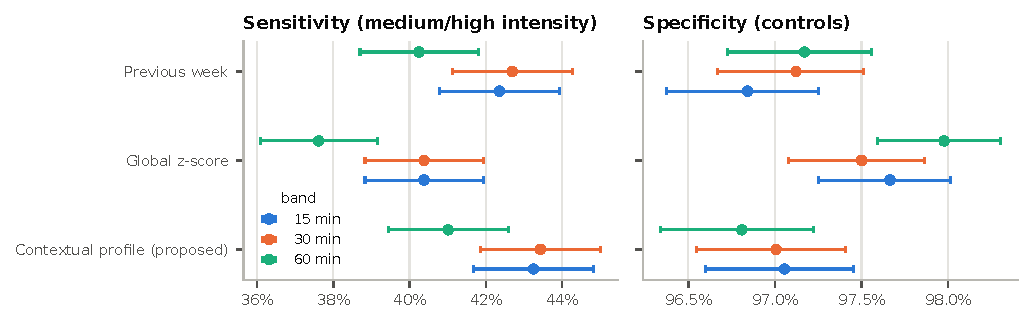
\includegraphics[width=0.85\textwidth]{figuras_en/fig_metodos.pdf}
  \caption{Sensitivity (medium and high intensities) and specificity by method and band, with 95\% Wilson CI.}
  \label{fig:metodos}
\end{figure*}

\paragraph{Operating point.} The limit of each indicator is its 99th percentile in the history (multiplier $c=1$), chosen because the query is only made when an incident is already open and a false \Residual diverts the operator's attention. Figure~\ref{fig:curva} also shows the points with 1\% and 2\% of alarms in the history: with 1\%, specificity rises to 99.0\% and sensitivity drops to 29.6\%. At these more conservative points, the baselines detect slightly more than the contextual profile (30.2\% and 30.8\%); at the adopted point, the three methods are equivalent.

\begin{figure}[t]
  \centering
  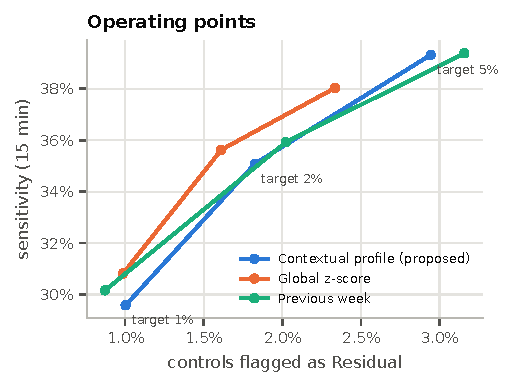
\includegraphics[width=0.85\columnwidth]{figuras_en/fig_curva_operacao.pdf}
  \caption{Sensitivity versus controls flagged as \Residual (15~min band), for targets of 1\%, 2\%, and 5\% of alarms in the history.}
  \label{fig:curva}
\end{figure}

\paragraph{By cause.} Sensitivity depends strongly on the cause (Figure~\ref{fig:sensmotivo}). Widespread system errors are detected in 59\% to 88\% of the cases, depending on the intensity, and 5xx errors from one consumer in 53\% to 62\%. Business errors are detected in 5\% to 34\% of the cases (widespread) and 13\% to 24\% (one consumer), because several resources already have high and variable 4xx rates. Latency ranges from 4\% ($\times$1.5) to 36\% ($\times$4) and reaches \textbf{61\%} [56, 66] for the 10-fold degradation.

\begin{figure}[t]
  \centering
  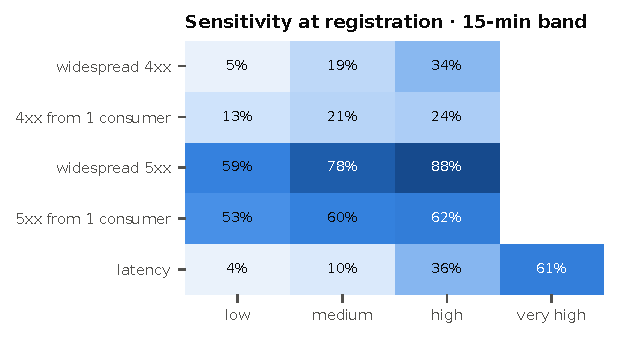
\includegraphics[width=0.9\columnwidth]{figuras_en/fig_sens_motivo.pdf}
  \caption{Sensitivity at registration (15~min band) by cause and intensity.}
  \label{fig:sensmotivo}
\end{figure}

\paragraph{By resource and by month.} By resource (Table~\ref{tab:recursos}), sensitivity ranges from 6\% (E10, with only two clients and real 5xx spikes) to 63\% (E09). By month, sensitivity was 49.8\% in August (7 resources) and 33.2\% in September (12 resources); restricted to the same 7 resources, September had 45.9\%. The drop in September therefore comes mainly from the resources that only enter in that month, with less history and more variation.

\paragraph{Band size and registration delay (RQ3).} The shortest band is the best when the incident is registered soon after the onset of the degradation (Figure~\ref{fig:atraso}): with a 15~min delay, sensitivity (medium and high intensities) is 45\% with the 15~min band, against 30\% with the 60~min band, which mixes normal and degraded minutes. With a 60 or 120~min delay, the 60~min band is slightly better (47--48\% against 42\%), because it reduces noise. On average, the 15 and 30~min bands are equivalent (43.2\% and 43.4\%) and superior to the 60~min band (41.0\%).

\begin{figure}[t]
  \centering
  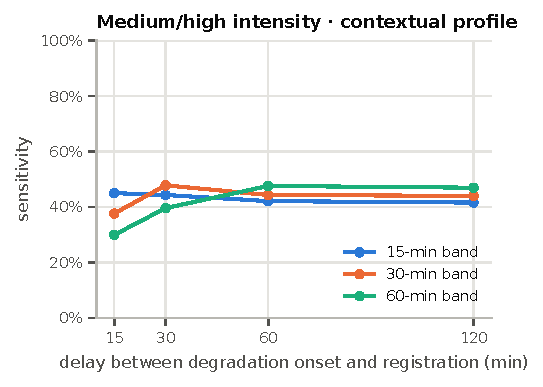
\includegraphics[width=0.85\columnwidth]{figuras_en/fig_sens_atraso.pdf}
  \caption{Sensitivity (medium and high intensities) by delay between the onset of the degradation and the registration, for each band size.}
  \label{fig:atraso}
\end{figure}

\subsection{Exp.~3: responsible indicator, onset, and scope (RQ2)}
When the resource is flagged as \Residual, the indicator pointed out is that of the injected cause in 96.5\% of the cases [95.7, 97.2] (Figure~\ref{fig:confusao}): 99.5\% for widespread 5xx, 97.7\% for 5xx from one consumer, 93.4\% for latency, and 91--92\% for 4xx. Accuracy is lower in E06 (69\%) and E02 (84\%), resources with a lot of natural variation in other indicators.

\begin{figure}[t]
  \centering
  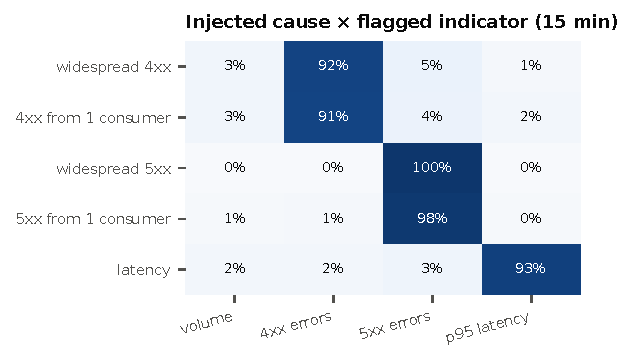
\includegraphics[width=0.85\columnwidth]{figuras_en/fig_confusao_indicador.pdf}
  \caption{Injected cause versus indicator pointed out (15~min band, detected cases).}
  \label{fig:confusao}
\end{figure}

The backward expansion (Figure~\ref{fig:expansao}) placed the actual onset within the estimated zone in 91.7\% of the detected cases [90.5, 92.7] (Table~\ref{tab:consulta}): 99\% when the degradation started 15 or 30~min before registration, 85\% with 60~min, and 83\% with 120~min (Figure~\ref{fig:inicio}). The errors are almost always underestimates: an intermediate band comes out \Normal, the search stops early, and the onset is estimated closer to the registration than it actually occurred.

\begin{figure*}[t]
  \centering
  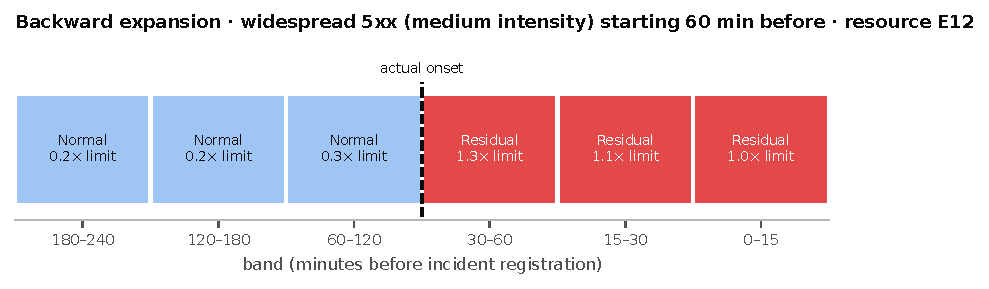
\includegraphics[width=0.85\textwidth]{figuras_en/fig_expansao_exemplo.pdf}
  \caption{Backward expansion in a widespread 5xx scenario that started 60~min before registration (E12): the three most recent bands are residual and the 60--120~min band is normal, and the onset is estimated between 30 and 120~min before.}
  \label{fig:expansao}
\end{figure*}

\begin{figure}[t]
  \centering
  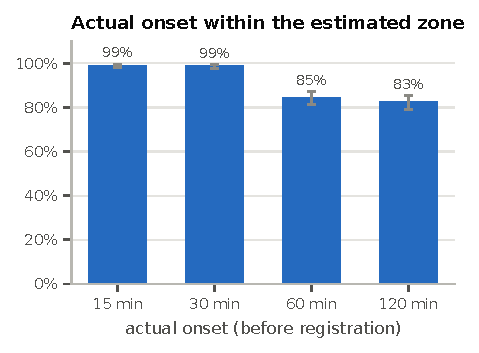
\includegraphics[width=0.8\columnwidth]{figuras_en/fig_inicio.pdf}
  \caption{Actual onset within the estimated zone, by delay (95\% Wilson CI).}
  \label{fig:inicio}
\end{figure}

\paragraph{Scope (complementary).} Among the 4xx and 5xx errors detected with the correct indicator, the scope was classified correctly in 76.3\% [74.3, 78.1]. Widespread errors are recognized as such in 85--90\% of the cases; those from one consumer, in 58\% (4xx) and 66\% (5xx).

\begin{table}[t]
  \caption{Exp.~3: quality of the query on the detected incidents (15~min band, 3-month history), in \% (95\% Wilson CI).}
  \label{tab:consulta}
  \small
  \begin{tabular}{lcc}
    \toprule
    Information & Cases & Hit \\
    \midrule
    Responsible indicator & 2,389 & 96.5 [95.7, 97.2] \\
    Onset in the estimated zone & 2,389 & 91.7 [90.5, 92.7] \\
    \quad degradation 15 or 30~min before & 1,245 & 99.0 \\
    \quad degradation 60 or 120~min before & 1,144 & 83.7 \\
    Scope (4xx and 5xx) & 1,911 & 76.3 [74.3, 78.1] \\
    \bottomrule
  \end{tabular}
\end{table}

\paragraph{Output for the agent and real event.} The query produces a structured document. Figure~\ref{fig:json} shows, in abridged form, the output of the scenario in Figure~\ref{fig:expansao}.

\begin{figure}[t]
\begin{Verbatim}[fontsize=\scriptsize,frame=single]
{"resource": "E12", "incident_registered": "2026-08-02 16:52",
 "context": {"day_type": "non-business", "hour": "16h"},
 "state": "Residual", "impacted_indicator": "5xx errors",
 "evidence": [{"indicator": "5xx errors", "observed": "15.7%",
    "normal_range_p5_p95": ["0.0%", "1.7%"], "times_limit": 1.02}],
 "estimated_onset": "between 30 and 120 min before registration",
 "scope": {"classification": "widespread",
    "active_clients": 27, "clients_with_errors": 10},
 "statistical_reason": "Resource E12 is outside the normal regime
   expected for a non-business day at 16h. Impacted indicator:
   5xx errors — 15.7% in the 15 min before registration (normal
   range 0.0% to 1.7%), 1.02× the resource's limit. The deviation
   started between 30 and 120 min before registration. The errors
   appear in 10 of 27 active consumers."}
\end{Verbatim}
\caption{Query output for the agent (abridged).}
\label{fig:json}
\end{figure}

In the real data, without injection, the query for E02 at 01:45 on September 2 returned \Residual due to 5xx errors: 4.1\% in the 15~min before registration (normal range from 0 to 1.1\%), in 15 of the 26 active consumers, with an onset estimated between 0 and 30~min before. E02 has a normal regime with high 5xx \emph{at 0h}; the event, one hour later, is outside it. It is a candidate real incident, to be confirmed with operations.

\subsection{Exp.~4: 3-month $\times$ 1-month history (RQ4)}
The longer history did \emph{not} improve the result (Table~\ref{tab:historico}, Figure~\ref{fig:historico}). With 1 month, sensitivity rose from 39.3\% to 42.1\% and specificity fell from 97.1\% to 96.3\%; in state hits, the 1-month history was better in all bands (McNemar: $p<0.001$ at 15, 30, and 60~min). The effect differs by month: in August, the 3-month history was slightly better in sensitivity (49.8\% against 47.8\%) and specificity; in September, the 1-month history detected considerably more (38.8\% against 33.2\%). The limits reflect this difference: with 3 months, the 4xx limit of E05 becomes 10 times larger, because the June to August history includes the high business error rate of July (3.2\%, against 0.8\% in August); the volume limit, in turn, is 18\% smaller at the median.

\begin{table}[t]
  \caption{Exp.~4: 3-month $\times$ 1-month history (15~min band, in \%; m/h = medium and high intensities).}
  \label{tab:historico}
  \small
  \begin{tabular}{lcccc}
    \toprule
    History & Sens. & Sens. m/h & Spec. & Ind. accuracy \\
    \midrule
    3 months & 39.3 & 43.2 & 97.1 & 96.5 \\
    1 month & 42.1 & 46.7 & 96.3 & 95.7 \\
    \bottomrule
  \end{tabular}
\end{table}

\begin{figure*}[t]
  \centering
  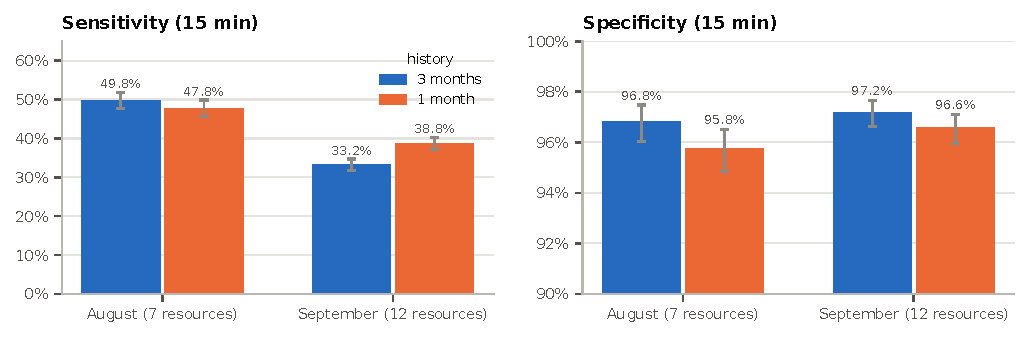
\includegraphics[width=0.85\textwidth]{figuras_en/fig_historico.pdf}
  \caption{Sensitivity and specificity by test month and history, with 95\% Wilson CI.}
  \label{fig:historico}
\end{figure*}

\subsection{Success criteria}
Four of the five criteria defined in business understanding were met (Table~\ref{tab:criterios}). Sensitivity was well below the target.

\begin{table}[t]
  \caption{Success criteria defined before modeling (15~min band, 3-month history).}
  \label{tab:criterios}
  \small
  \begin{tabular}{p{0.5\columnwidth}p{0.22\columnwidth}c}
    \toprule
    Criterion & Result & Met \\
    \midrule
    Controls with \Normal output $\geq$ 95\% & 97.1\% & yes \\
    Sensitivity (medium/high) $\geq$ 70\% & 43.2\% & no \\
    Indicator accuracy $\geq$ 90\% & 96.5\% & yes \\
    Actual onset in the estimated zone $\geq$ 70\% & 91.7\% & yes \\
    No significant loss to the baselines & no loss & yes \\
    \bottomrule
  \end{tabular}
\end{table}

%% =====================================================================
\section{Discussion}\label{sec:discussao}

\paragraph{RQ1: regimes and state at registration.} The aggregated AALs show clear regimes tied to the context in all resources, especially to the hour: batches, business hours, early morning, and even normal regimes with high errors at specific hours. The contextual profile decides the state of each resource at the moment of the incident with high specificity (97.1\%). In the main band, however, it ties with the global z-score and with the previous week; the detection gain from the context is small and only appears in the 30~min band. This does not make the context useless; its clearest contribution is the \emph{explanation}, with the definition of the normal range of the context, the expected regime, and the limit of each indicator. This is what makes it possible to tell the operator ``4.1\% of 5xx at 1h, when normal is up to 1.1\%''. For the operator, a \Residual result is strong information: it rarely appears without reason and comes with the right indicator; a \Normal result indicates that the resource is unlikely to be the problem, but does not rule out subtle degradations.

\paragraph{The limit per indicator.} The main modeling decision was to normalize each indicator by its own tail in the resource. Without it, with indicators that have frequent real spikes, as in the business errors of resources E04, E05, and E07, the defined threshold may hide deviations in latency and system errors. In real AALs, the indicators do not have the same variability, and a single global threshold over all of them tends to encompass the noisiest ones.

\paragraph{RQ2: indicator and onset.} The strongest point of the method is the quality of the information when it is issued: the responsible indicator is pointed out correctly in 96.5\% of the cases, and the onset is located in the right zone in 91.7\%. The backward expansion is simple to explain, looking back until a normal period is found, and gives the operator a useful answer.

\paragraph{RQ3: band size.} The 15~min band is the best choice as the main decision, because the incident is usually opened shortly after the onset of the degradation. Larger bands only pay off when the degradation has already lasted an hour or more. In practice, the short band decides the state and the backward expansion provides the horizon.

\paragraph{RQ4: how much history.} More history did not mean a better profile. APIs shift level over the months, with volume growing and business error rates changing, and a three-month history includes behaviors that no longer hold, which widens the limits. The 1-month history gained mainly in September, when the change was greatest. For deployment, this points to frequent retraining with recent history instead of accumulating months.

\paragraph{Latency and less sensitive resources.} With the 10-fold degradation, latency is detected in 61\% of the cases, against 36\% with 4-fold. The p95 of the per-minute means has heavy tails even on normal days, exceeding 10 times the median of the context, which forces high limits; a per-request percentile, if available in the gateway, is the natural path for improvement. Resources with frequent real spikes in an indicator receive high limits for it, and only large deviations appear, as is the case of resources with a high number of business errors. In these cases, the limit itself is useful information: it tells the operator that the indicator is already unstable for the resource.

%% =====================================================================
\section{Threats to validity}\label{sec:ameacas}

\paragraph{Synthetic faults.} The performance measures the ability to detect \emph{the injected causes}, not real failures. The varied intensities, the four delays, the two months, and the large number of scenarios reduce, but do not eliminate, this bias. The accuracy of the indicator, the onset, and the scope is measured only on detected incidents, which tend to be the strongest ones.

\paragraph{Method parameters.} The operating point (limit at the 99th percentile, $c=1$) and the latency intensity $\times$10 were fixed without optimization on the test scenarios. The $\times$10 intensity is justified by the distribution of the history, and the lower intensities are reported. In k-means, the indicators were capped at the 1st and 99th percentiles so that isolated spikes would not form trivial clusters; since k-means is descriptive, this does not affect the decision metrics. The main history (3 months) was fixed before observing the results, and the result unfavorable to it is reported.

\paragraph{Controls and real anomalies.} The control queries use real data without injection, which may contain real anomalies (such as the one in E02), counted as false \Residual. Specificity is therefore a conservative estimate.

\paragraph{Approximate latency.} The p95 is computed over the means per minute and per client, not over requests; the real tail tends to be larger. A latency 10 times higher could, in practice, hit the gateway \emph{timeout} and become a 504 error, which the injection does not simulate.

\paragraph{Generalization.} The results come from one organization and 12 resources. The dataset cannot be shared; the notebook code is independent of the data.

%% =====================================================================
\section{Final remarks}\label{sec:conclusao}

This work showed that Access Logs aggregated per minute, without \emph{traces} or application logs, make it possible to characterize the normal regimes of each API resource and to report, at the moment an incident is opened, whether the resource is in a normal or residual regime, which indicator was impacted (business errors, system errors, or latency), and since when. The method uses simple techniques, such as median, MAD, percentiles, cross-validation, and a backward search, requires no labels, and produces an explanation of the context that an agentic system or operator can use directly.

In two months of testing, the information was reliable when issued: 97.1\% specificity, 96.5\% indicator hits, and 91.7\% hits in the onset zone. Sensitivity is still limited, around 40\%: relatively high for system errors, moderate for large latency degradations, and low for business errors in resources with many natural 4xx. It also showed that the backward expansion complements the information with the onset of the deviation, which is also useful for the context of the incident. The recent 1-month history proved better than the long 3-month one, which recommends frequent retraining with a smaller volume of data.

As future work, we highlight: (i) validating the method with real incidents and with the assessment of operators; (ii) improving sensitivity to latency with per-request percentiles; (iii) exploring other data mining techniques to improve sensitivity; and (iv) integrating the query as a tool of an incident support agent.

\bibliographystyle{ACM-Reference-Format}
\bibliography{referencias_en}

\end{document}
